% Chapter 1

\chapter{Introducción general} % Main chapter title

\label{Chapter1} % For referencing the chapter elsewhere, use \ref{Chapter1} 
\label{IntroGeneral}

%----------------------------------------------------------------------------------------

% Define some commands to keep the formatting separated from the content 
\newcommand{\keyword}[1]{\textbf{#1}}
\newcommand{\tabhead}[1]{\textbf{#1}}
\newcommand{\code}[1]{\texttt{#1}}
\newcommand{\file}[1]{\texttt{\bfseries#1}}
\newcommand{\option}[1]{\texttt{\itshape#1}}
\newcommand{\grados}{$^{\circ}$}

%----------------------------------------------------------------------------------------

En este capítulo se explican las causas que dan origen al dispositivo desarrollado y la función que este cumple en el proyecto de la empresa Skyloom Global. Se hace una breve descripción de un amplificador óptico, del hardware ya existente y por último se presentan los objetivos y alcances determinados durante la planificación de este trabajo.


%----------------------------------------------------------------------------------------
\section{Contexto de la empresa}
\label{sec:contexto}

La creciente demanda de mayores velocidades de transmisión de información en el ámbito aeroespacial, combinada con las limitaciones de la radiofrecuencia, favorecen el surgimiento de nuevas empresas enfocadas en el desarrollo de nuevas tecnologías capaces de superar estas barreras. Tal es el caso de la empresa Skyloom Global, que propone la creación de una red de satélites de órbita baja (LEO) \citep{WEBSITE:LEO} utilizando enlaces ópticos de alta velocidad.

El funcionamiento general de esta idea se basa en un satélite geoestacionario (órbita GEO) \citep{WEBSITE:GEO} al cual los satélites en LEO transmiten la información (denominado \textit{uplink}) para luego descargar esta a una estación en Tierra (denominado \textit{downlink}). De esta forma se obtiene una alta disponibilidad de los datos ya que el satélite en GEO siempre tiene visión de la Tierra. Un diagrama de esta propuesta se muestra en la figura \ref{fig:propSky}.

\begin{figure}[H]
\centering
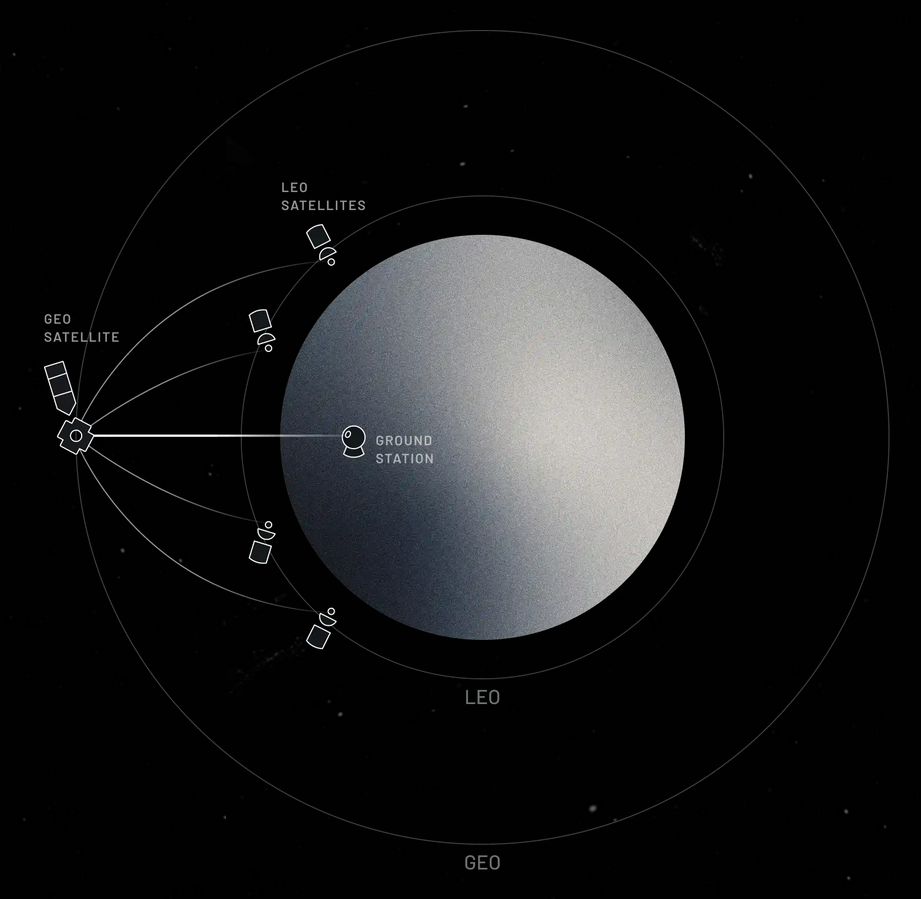
\includegraphics[width=0.8\textwidth]{./Figures/propuesta_skyloom.png}
\caption{Propuesta de la empresa Skyloom Global\protect\footnotemark.}
\label{fig:propSky}
\end{figure}

\footnotetext{Imagen tomada de \url{https://www.skyloom.co/}}

El enlace óptico, que permite la transmisión y recepción de datos a una velocidad de 1 Gbps (1 \textit{Gigabit} por segundo) entre satélites, se establece mediante una terminal de comunicaciones óptica, que es el principal producto actualmente en desarrollo por la empresa. Estas terminales cuentan con un láser que trabaja sobre una longitud de onda de 1550 nm (banda C del espectro). Dicho láser es el encargado de transmitir la información propiamente dicha mediante pulsos de luz (no visible).

En líneas generales los láseres de esta longitud de onda que se encuentran en el mercado no cuentan con la potencia óptica necesaria para que en el receptor se la detecte. Esto se debe principalmente a que la distancia de espacio libre estimada entre dos satélites en LEO es de unos 4000 km \citep{WEBSITE_SKY}.

Para solucionar el problema antes mencionado se introduce a la salida del láser un amplificador dopado con erbio o EDFA (de las siglas \textit{Erbuim Doped Fiber Amplifier}) \citep{WEBSITE:EDFA2}. La función de este dispositivo es aumentar la potencia del láser varias veces de forma que se alcance un nivel adecuado para la transmisión.

El modelo de amplificador utilizado por la empresa cuenta con un conector que provee una interfaz electrónica para poder controlar su funcionamiento. Esta interfaz cuenta con distintas señales y buses de comunicación que se explican con mayor detalle en la sección \ref{sec:intAmp}.

Este amplificador formará parte de la terminal de comunicaciones y estará sometido a intensivas pruebas de funcionamiento y rendimiento durante la etapa de investigación y desarrollo. Para esto es indispensable contar con una herramienta que brinde a los ingenieros a cargo de estas la posibilidad de utilizar el amplificador de forma aislada, es decir, sin tener que usar hardware perteneciente al producto final.

En la figura \ref{fig:bloquesProy} se puede ver un esquema de uso del dispositivo junto con las conexiones con el hardware externo.

\begin{figure}[H]
\centering
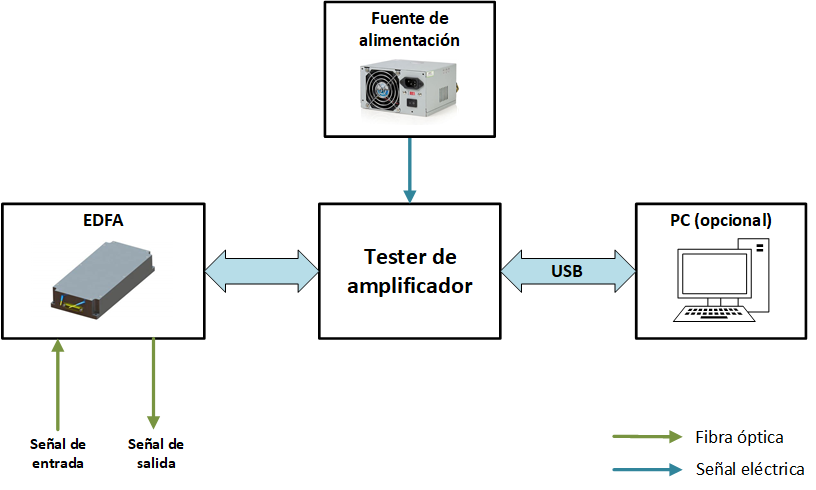
\includegraphics[width=0.85\textwidth]{./Figures/bloquesProy.png}
\caption{Esquema de uso y conexionado del sistema.}
\label{fig:bloquesProy}
\end{figure}

El dispositivo cuenta con tres conexiones externas: la interfaz con el amplificador, la conexión a la fuente de alimentación y un puerto USB.

La interfaz con el EDFA permite controlarlo y consultar diversos parámetros de funcionamiento a través de las señales presentes en el conector. La fuente de alimentación se encarga de energizar el tester y el EDFA. Y por último, la conexión USB permite controlar el amplificador del mismo modo que en el tester, por lo que el uso de la PC es opcional. Para poder hacer esto, sobre esta debe correr un software que permita establecer una comunicación.

%----------------------------------------------------------------------------------------

\section{Estado del arte}

Actualmente el fabricante del amplificador posee a la venta una placa electrónica capaz de conectarse a un EDFA y proveer ciertas funcionalidades similares. La empresa ha hecho uso de ella en el pasado pero luego pasó a descartarla debido a tres problemas mayores:

\begin{itemize}
\item No permite el uso de todas las señales presentes en el conector del amplificador.
\item Tiene una tasa de fallas muy alta, en particular la interfaz UART.
\item Su costo es muy elevado en relación a sus prestaciones.
\item El tiempo de entrega del producto es de varias semanas.
\end{itemize}


\section{Motivación}

Las desventajas expuestas en la sección anterior son los principales motivos que dieron origen a la necesidad de contar con el sistema propuesto en este trabajo. Esto le permite a la empresa no depender del fabricante para la entrega de estos testers y por lo tanto reducir costos y tiempos.

Por otro lado, el dispositivo diseñado en este trabajo no solo cuenta con las mismas funcionalidades que el del fabricante si no que ademas posee las que este no tiene y otras características adicionales que lo hacen mas fácil de usar y menos propenso a fallas.

%----------------------------------------------------------------------------------------

\section{Objetivos y alcance}

El objetivo principal de este trabajo fue el desarrollo de un dispositivo capaz de controlar y realizar mediciones sobre un amplificador de fibra óptica. Las tareas contempladas fueron:

\begin{itemize}
\item Diseño y construcción de un prototipo funcional del dispositivo.
\item Diseño e implementación del firmware del dispositivo.
\item Diseño de los bancos de prueba y ensayos.
\item Simulación del funcionamiento del hardware mediante software.
\item Documentación de diseño y manual de uso.
\end{itemize}

Los puntos del desarrollo que no se contemplaron en el trabajo fueron:

\begin{itemize}
\item Diseño y construcción de la versión final del dispositivo.
\item Especificación de las pruebas a ejecutar sobre el amplificador óptico utilizando el dispositivo.
\item Fabricación del PCB del dispositivo.
\item Procesamiento e interpretación de los valores de los parámetros del EDFA.
\item Diseño y construcción de la fuente de alimentación externa.
\item Diseño e implementación del software a ejecutarse en la PC.
\end{itemize}


%----------------------------------------------------------------------------------------
